\section{Statistical Framework} \label{sec:stat_fra}
This section illustrates the concepts and notations defined in \cite{dbb1}.
\subsection{General notations}

In this paper, all random variables are defined on a probability space $(\Omega,\mathscr{A},P)$. The expected value and variance/covariance operators are defined with respect to the probability measure $P$. 
For two sets $E$ and $F$, $(E\to F)$ or $F^E$ designate the set of the functions from $E$ to $F$.
The notation "$g:E\to F,x\mapsto g(x)$" means: let $g$ be a mapping from set $E$ to set $F$ that to $x$ associates $g(x)$. For $f:E\to (F\to G)$, $g:E\to F$, $h:E\to (H\to F)$,  the notation $f[g]$ designates the function :  $f[g]:E\to G$, such that $f[g](x)=(f(x))(g(x))$, and the notation 
$f[h]$ designates the function :  $f[h]:E\to (H\to G)$, such that $f[h](x)=(f(x)\circ h(x))$.


For a set $E$, $\bar{E}$ designates the set $\{\mathbf{0}\}\cup\bigcup_{n\in\mathbb{N},n\geq 1} E^{\{1,\ldots,n\}}$, where $\mathbf{0}=E^\emptyset$ corresponds to the set containing an application with empty domain.
Let denote by $\size $ the application that maps an application to the cardinality of its domain: $\bar{E}\to\mathbb{N}$, $\mathbf{e}\mapsto n$ if $\position\in E^{\{1,\ldots,n\}}$, $0$ if $\position=\mathbf{0}$. For an application $\position\in\bar{E}$, a set $\Sampleindex$, $\position_\Sampleindex$ is the application:
$\position_\Sampleindex:\Sampleindex\cap\mathrm{domain}(\position)\to E:\ell\mapsto\position(\ell)$, in the case of a random application $\Sample:\Omega\to\toPop$ and a random set :$\Sampleindex\to(\mathscr{P}(\mathbb{N})$ ($\mathscr{P}(\mathbb{N})$ is the set of all subsets of $\mathbb{N}$), then $\Sample_\Sampleindex$ is the random application: $\Omega\to\toPop, 
\omega\mapsto 
\Sample_\Sampleindex(\omega):(\Sampleindex(\omega)\cap\mathrm{domain}(\Sample(\omega))\to \Pop),
\ell\mapsto (\Sample(\omega))(\ell)$.
For a measure $\eta$ of $E$, a non random finite set $\Sampleindex$, $\eta^{\otimes\Sampleindex}$ is the measure such that for any collection $(\subsetA_\ell)_{\ell\in\Sampleindex}$ of subsets of $E$  :
$\eta^{\otimes\Sampleindex}\left(\bigcap_{\ell\in\mathbb{L}}\{\position\in E^\Sampleindex:\position(\ell)\in\subsetA_\ell\}\right)=\prod_{\ell\in\Sampleindex}\eta(\subsetA_\ell)$, and
$\eta^{\otimes\emptyset}(\{\mathbf{0}\})=1$, 
then define the measure $\bar{\eta}$ on $\bar{E}$: $\bar{\eta}=\eta^{\otimes\emptyset}+\sum_{\samplesize\in\mathbb{N},\samplesize\geq 0}\eta^{\otimes\{1,\ldots,\samplesize\}}$.

\subsection{Spatial process}
We consider a space $\Pop$, that is a compact (non necessarily convex) subset of a finite dimensional real vector space $\mathbb{R}^d$, with its associated Borel sigma-field, and a random process $\Signal$ defined on $\Pop$ with value in another finite dimension real vector space $\SignalSpace$, e.g. $Y:\Omega\to(\Pop\to\SignalSpace)$.
 For example for a random variable $\Sample:\Omega\to\Pop^{\{1,2\}}$, and a random variable
$\Signal:\Omega\to(\Pop\to\SignalSpace)$, 
$\Signal[\Sample]$ is the random variable: $\Signal[\Sample]:\Omega\to(\{1,2\}\to\SignalSpace)$, $\omega\mapsto(\Signal(\omega))(\Sample(\omega)):\ell\to(\Signal(\omega))(\Sample(\omega)(\ell)$.
The set of all functions 
All definitions will be given under the general statistical framework described above. Examples and illustrations will be given for the particular case where $\Pop=[0,1]^2$.
%Given data $(\position(1),\signal_{1}),...,(\position_{n},\signal_{n})$, in order to perform inference for some target, we postulate a model, which we assume holds for the entire population. In particular, we are interested in model parameters, in other words we focus on \emph{analytic inference}. The choice of the model is not an easy task. It should reflect the structure of the population and should capture the important features useful for inference purpose. An entire branch of literature is dedicated to this task, i.e. \emph{model selection}, but the focus of this paper does not lie in that. 
%For our work we assume that the model describing the variable of interest is given by
%\begin{equation} \label{eq:model}
%\Signal\left[\position\right]=S\left[\position\right]+\epsilon\left[\position\right]
%\end{equation}
%{\color{red} S is for $\Sample$ (sample)}
%where $S\left(\position\right)$ is a zero mean stationary stochastic process in $\mathbb{R}^d$ and is independent from the $\epsilon\left(\position\right)$, which has normal distribution with mean 0 and variance $\sigma_{\epsilon}$. The model in \eqref{eq:model} is quite general and embraces many variations under its umbrella. It is wide known in the field of geostatistics, where the term \emph{kriging} is in vogue. In fact, according to different assumptions about $S(\position)$, we end up with different models, which are usually referred with terms as ordinary kriging, simple kriging, universal kriging and so on. In order to perform inference about the model parameters, we need to introduce some assumptions.
Let $\dominantY$ (resp. $\dominantU$) denote a sigma-finite measure on the set $\SignalSpace$ (resp. $\Pop$).
The notation $\density_{V\mid W}$ denotes the density of $V$ conditional on $W$ with respect to a dominating measure on the domain of $V$.
The average theoretical semivariogram is defined as the function: 
\begin{equation}\Semivariogram:\mathbb{R}^d\to[0,+\infty),h\mapsto\frac12\int_{\Pop^{\{1,2\}}} \Var\left[\Signal[\position(2)]-\Signal[\position(1)]\right] \derive(\dominantU^{\otimes \{1,2\}})^{X\mid X[2]-X[1]=h}(\position),\label{eq:averagesemivariogram}\end{equation} 
where $(X)$ is the identity of $\Pop^{\{1,2\}}$, and the average theoretical covariogram is the function  $\nu^{X_2-X_1}-a.s(h)$-defined:
\begin{equation}\Covariogram:\mathbb{R}^d\to\mathbb{R}, h\mapsto\int_{\Pop^{\{1,2\}}} \Cov\left[\Signal[\position(1)],\Signal[\position(2)]\right] \derive(\dominantU^{\otimes \{1,2\}})^{X\mid X[2]-X[1]=h}(\position).\label{eq:averagecovariogram}\end{equation} The covariogram and semivariogram satisfy the relationship: $\forall h\in\mathbb{R}^d, \Semivariogram(h)=\Covariogram(0)-\Covariogram(h)$.

%The functions $\Covariogram$ and $\Semivariogram$ satisfy the relationship:
% $$\Covariogram(h)=\Covariogram(0)-\Semivariogram(h)$$.
\begin{definition}[Intrinsic stationarity and Second order stationarity, \protect{\citep[p.~53]{cressie2015statistics}}]
A process is intrinsic stationary when the following conditions are satisfied :  $\forall \position\in\Pop^{\{1,2\}}$,
\begin{eqnarray}
    \mathrm{E}\left[\Signal\left[\position(2)\right]-\Signal\left[\position(1)\right]\right]&=&0\\
    \frac12~\Var\left[\Signal\left[\position(2)\right]-\Signal\left[\position(1)\right]\right]&=&\Semivariogram(\position(2)-\position(1))\label{eq:semivariogram}
\end{eqnarray}
A process is second order stationary when the following are satisfied:
\begin{equation}
\exists\mu\in\mathbb{R},~    \forall\position\in \Pop,~~ E\left[\Signal\left[\position\right]\right]=\mu
\end{equation}
\begin{equation} \label{eq:covariogram}
    \forall~\position\in \Pop^{\{1,2\}}, ~\Cov\left[\Signal\left[\position(1)\right],\Signal\left[\position(2)\right]\right]=C\left(\position(1)-\position(2)\right)
\end{equation}
\end{definition}
%The function $\Covariogram\left(\cdot\right)$ in \eqref{eq:covariogram} is called \emph{covariogram}, or \emph{stationary covariance function}. 
In the case of a first order stationary process, the variance operator $\Var[.]$ can equivalently be replaced by the square expected value opeartor $\mathrm{E}[(.)^2]$ in equation \eqref{eq:averagesemivariogram}.
In the case of a second order stationary process, equations \eqref{eq:averagecovariogram} and \eqref{eq:averagesemivariogram} correspond to the definition of the theoretical covariogram and semivariogram as found in \citet[p.~53 and p.~58]{cressie2015statistics}.
The random process is isotropic if in addition on being second order stationary, the covariogram function $h\mapsto \Covariogram(h)$ only depends on $h$ via $h\mapsto\|h\|$.

%{\color{red} Let us call $\gamma$ the parameters for the Semivariogram or $c$ the parameters for the Covariance.
%A plot of the 4 variograms would be neat there. Throughout the paper, $c_0$ should be replaced by $\sigma$}

Common model assumptions on the process $\Signal$ consist in assuming second order stationarity and isotropy. Covariance structure of the signal is then fully characterized by $\Covariogram(0)$ and $\Semivariogram(h), h\neq 0$. 
%We give the  covariogram formal expression for a list of covariogram models. 
A Gaussian covariogram is 
a function of the form:
$h\mapsto\Covariogram(h)=c_0+c_1\left(1-\exp\left(-\|h\|^2/(2c_2^2)\right)\right)$ where $c_0,~c_1,~ c_2\in[0,+\infty)$
(see \cite[p.~80]{chiles1999geostatistics} for more models). 
%For $h\in\mathbb{R}^d$, $\|h\|>0$:

%\begin{table}[H]
%\setlength{\tabcolsep}{28pt}
%\renewcommand{\arraystretch}{1.8}
%\caption{Covariograms}
%\begin{tabular}{lll}
%\hline
%($\Semivariogram\left(h\right)$)&Parameters&Type\\
%\hline
%\hline
%$c_{0}+c_1\|h\|$& $c_0,~c_1\in[0,+\infty)$&Linear\\
%%\hline$\begin{array}{ll}c_{0}+c_{s}\lbrace\left(3/2\right)\left(h/a_{s}\right)-\left(1/2\right)\left(h/a_{s}\right)^{3}& \text{ if } 0<h\leq a_{s},\\
%%    c_{0}+c_{s}&\text{ if } h\geq a_{s}\end{array}$&&
%% Spherical\\
%\hline    $c_0+c_1\left( 1-\exp\left(-\|h\|/c_2\right)\right)$&$c_0,~c_1,~ c_2\in[0,+\infty)$&Exponential\\
%\hline
%$c_0+c_1\left(1-\exp\left(-\frac{\|h\|^2}{2c_2^2}\right)\right)$&$c_0,~c_1,~ c_2\in[0,+\infty)$&Gaussian\\
%\hline
%\end{tabular}
%\end{table}

%If $\gamma$ is continuous in $0$, $\gamma(0)=0$
\subsubsection*{Example with simulations: isotropic Gaussian process $\Signal$.}
In the case where $\Signal:\Omega\to(\Pop\to\SignalSpace)$ is a Gaussian random process, its distribution  can be derived from the distributions of $\Signal[\position]$, where $\position\in\toPop$. 
For $\position$, $\position'\in\toPop$, denote the expected value of the signal by $\mu:\toPop\to\toSignalSpace,\position\mapsto\mathrm{E}\left[\Signal[\position]\right]$, and the covariance of the the random vectors $\Signal[\position]$, $\Signal[\position']$  by $\provar_{\position,\position'}=\Cov \left[\Signal[\position],\Signal[\position']\right]$.
The distribution of $\Signal$ is then fully characterized by $\mu$ and $\provar$: for $n\in\mathbb{N}$,   $\position\in\Pop^{\{1,\ldots,\samplesize\}}$, $\Signal[\position]$ has the following density with respect to $\dominantY^{\otimes \{1,\ldots,n\}}$: 
%As first example, we present a spatial Gaussian process. A \emph{Gaussian process} is a stochastic process, such that every finite collection of those random variables has a multivariate normal distribution. Hence, given the model \eqref{eq:model}, we assume 
%$\Signal\sim\mathcal{N}\left(0,\provar\right)$. In this scenario the probability density function is given by: for $n\in\mathbb{N}$, $\position\in\Pop^n$,  
\begin{equation} \label{eq:pdf_norm_process}
    \density_{\Signal[\position]}\left(\signal\right)=\left(2\pi^{n/2}|\provar_{\position,\position}|^{\frac12}\right)^{-1}\exp\left(-\frac12(\signal-\mu(\position))\provar_{\position,\position}^{-1}(\signal-\mu(\position))^{\!\mathrm{T}}\right).
\end{equation}
In the case of an isotropic Gaussian process, the 
distribution of $\Signal$ is fully characterized by $\mu$ and $\Semivariogram$.
%and the respective likelihood for a sample of dimension $n$ is
%\begin{equation} \label{lik_norm_process}
%   \mathcal{L}_{\Signal[\position]}\left(\parampop;\signal\right)=\density_{\left(\Signal\left[\position\right];\theta\right)}\left(\signal;\theta\right)
%\end{equation}
%\input{prc_y.tex}
We simulate three independant replications of an isotropic Gaussian process with $\Signal:\Omega\to(\Pop=[0,1]^2\to\mathbb{R})$, with $\forall \position\in\Pop$, $\mathrm{\mu}[\position]=0$ and with a Gaussian Covariogram with parameters
 $c_0=0$, $c_1=5$, $c_2=10$.
Figure \ref{fig:oaijsfdoij} represents the independent realizations of $\Signal$.
\begin{figure}[H]
%\begin{mdframed}

    \caption{Heat maps of realisations of the random process $\Signal:\Omega\to(\Pop=[0,1]^2\to\mathbb{R})$}
    \label{fig:oaijsfdoij}
    
\hspace{-.6cm}\includegraphics{fig/figure1.pdf}

    \vspace{-.4cm}
    {\footnotesize For each realisation $\signal$ of the random process $\Signal$, for each $\position$ in $\Pop$, the value of $\signal[\position]$ is color coded with a grayscale gradient.}
%\end{mdframed}
\end{figure}




\subsection{Sample, design and design variable} \label{sec:design}

\subsubsection{Fixed designs and design variables}

By definition a design $\design$ is a probability distribution on $\toPop$.
A sample $\Sample$ drawn from $\design$ is a random variable or point process of distribution $\design$, e.g. a random variable $\Sample$ such that $\mathrm{P}^\Sample=\design$. 
Define the size $\Samplesize=\mathrm{size}\circ\Sample$ of the sample $\Sample$. The sample density with respect to $\dominantUbar$, is defined by:
$(\derive P^\Sample)/(\derive\dominantUbar)(\position)=P(N=n)\times(\derive P^{\Sample\mid N=n})/(\derive\dominantU^{\otimes\{1,\ldots,n\}})(\position)$, if $\position\in\Pop^{\{1,\ldots,n\}}$, $P(N=0)$ if $\position=\mathbf{0}$. 
%For example, let $\intensity:(\Pop,\dominantU)\to(\mathbb{R}^+,\mathrm{Lebesgues}(\mathbb{R}^+))$ be a measurable function , then a Poisson point process \citep[p.~ 45]{CoxIshamPointProcesses}) with intensity $\pi$ follows a finite or discrete design if the support of $\dominantU$ is finite. The distribution of a Poisson process when the support of $\dominantU$ is finite is a design that corresponds to with replacement sampling. Confusingly, in the literature on survey sampling, Poisson sampling \citep[p.~85]{SarndalSwensonWretman1992} corresponds to a finite design where each unit $\position$ such that $\pi(\position)>0$ is drawn independently with a fixed probability $\pi(\position)$, and is thus a without replacement design.
A fixed design variable is a function $\desvar:\Pop\mapsto \DesvarSpace$.
A fixed size design $\design$ is usually defined as a function of a fixed design variable, and characterised by its density with respect to $\dominantUbar$. For example, 
the Probability Proportional to Size $\desvar$ With Replacement and size $n$ ($\mathrm{PPSWR}(\desvar,n)$) design, with $\DesvarSpace=[0,+\infty)$ is characterized by:  
\begin{equation}\label{eq:ppswr}\left(\derive P^{\Sample}/\derive\dominantUbar\right)(\position)=\left(\int_U \left(\desvar[\position']\right)\mathrm{d}\dominantU (\position')\right)^{-\samplesize}
\left(\prod_{\ell=1}^\samplesize\left(\desvar[\position(\ell)]\right)\right)\text{ if }\position\in\Pop^{\{1,\ldots,n\}},~0\text{ otherwise.}
\end{equation}
The point process $\Sample$ characterized by Equation \eqref{eq:ppswr} is a binomial point process of $\samplesize$ points in $\Pop$ with intensity $\Pop\to\mathbb{R}, \position\to\left(\left(\desvar.\dominantU\right)\left(\Pop\right)\right)^{-1}\desvar[\position]$, which we abbreviate by $\Sample\sim\mathrm{bpp}\left(\desvar,10\right)$. Simple random sampling with replacement is a binomial point process with a constant intensity.  For simplicity, we only consider exchangeable sample designs, in the sense that $\forall \samplesize\in\mathbb{N}$, for all permutation $\permutation$ of $\{1,\ldots,n\}$. $P^{S\mid\Samplesize=\samplesize}=P^{S[\permutation]\mid \Samplesize=\samplesize}$. %Pdesigns such that: 
%This general definition includes design for with and without replacement sampling and fixed and random size sampling. 
For example, given a measurable real function $\desvar :\Pop \to\mathbb{R}$, a spatial Poisson Process of intensity $\desvar$ is a point process 
$S:\Omega\to\bigcup_{\samplesize\in\mathbb{N}}\Pop^{\samplesize}$, such that 
for all $\dominantU$-measurable subset $\subsetA$ of $\Pop$, \begin{equation}\label{eq:poissonprocess}
S\sim\mathrm{Ppp}(\desvar)\Leftrightarrow
\mathrm{cardinality}(\Sample^{-1}[\subsetA])\sim \mathrm{Poisson}\left((\desvar.\dominantU)\left(\subsetA \right)\right),
\end{equation}

where $\Sample^{-1}[\subsetA]$  is the random variable with domain the finite subsets of $\Pop$ defined by: $\omega\mapsto\{\ell\in\{1,\ldots,\Samplesize(\omega)\};(\Sample(\omega))(\ell)\in \subsetA\}$ if $\Samplesize(\omega)>0$, $\emptyset$ otherwise.

The density of such process with respected to $\bar\dominantU$ is defined, for $\samplesize\in\mathbb{N}$, $\position\in \toPop$, by:
\begin{equation}
\density_{\Sample}(\position)=\left(\size (\position)!\right)^{-1}\exp\left(-\left(\desvar.\dominantU\right)(\Pop)\right)
\prod_{\ell\in\mathrm{domain}(\position)}
\desvar[\position(\ell)].
\end{equation}



%
%The Poisson Point process is such that for two measurable subsets $\subsetA_1$ and $\subsetA_1$  of $\Pop$, 
%$\subsetA_1\cap\subsetA_2=\emptyset\Rightarrow \left(\mathrm{\cardinality}(\subsetA_1\cap\Sample)\perp\mathrm{\cardinality}(\subsetA_2\cap\Sample))$, which is not necessarily the case for each Point Process (for example fixed strictly positive size point processes

%When there exists $\position(1),\ldots,\position_N\in\Pop$ such that $\dominantU=\mathrm{Dirac}_{\{\position(1),\ldots,\position_N}\}$, simple random sampling is  is finite and 

%
%Tables {\ref{tab:oiurhgoieruhgierug}} and 
%\ref{tab:oijgoirejoier} provide examples of continuous and finite population designs. 
%%Notice that the same name is used in the literature for finite or continuous population designs, without contradiction. We put them there as one goal is to establish a parallel between existing theoretical work between finite population and continuous population sampling.
%
%\begin{table}[H]\label{tab:oiurhgoieruhgierug}
%\caption{Continuous population fixed size designs}
%
%\small
%\setlength{\tabcolsep}{8pt}
%\renewcommand{\arraystretch}{1.8}
%
%\newcolumntype{b}{X}
%\newcolumntype{s}{>{\hsize=.1\hsize}X}
%
%\begin{tabularx}{\textwidth}[t]{ssb}
%\hline
%\multicolumn{3}{p{\dimexpr\linewidth-\tabcolsep-\arrayrulewidth}}{Name}\\                 &$\DesvarSpace$ & $\mathrm{d} P^{\Sample[\{1,\ldots,n\}]}/\mathrm{d}\dominantU^{\otimes n}(\position)$\\
%\hline
%\hline
%\multicolumn{3}{p{\dimexpr\linewidth-\tabcolsep-\arrayrulewidth}}{Probability Proportional to Size $\desvar$ With Replacement (PPSWR)}\\                 & $[0,+\infty)$ & $\left(\int_U \left(\desvar[\position']\right)\mathrm{d}\dominantU (\position')\right)^{-n}
%\left(\prod_{\ell=1}^n\left(\desvar[\position(\ell)]\right)\right)$\\
%\hline 
%\multicolumn{3}{p{\dimexpr\linewidth-\tabcolsep-\arrayrulewidth}}{Sytematic sampling, $\samplesize=(n')^2$ }\\&$\{1\}$                 &
%$\left\{\begin{array}{ll}(n!)^{-1} n &\text{ if }\position\in\left\{(\position_0+(n')^{-1}\alpha)_{\alpha\in \{0,\ldots,n'-1\}^2}\mid\position_0\in [0,1/n']^2\right\}\\0& \text{ otherwise.}\end{array}\right.$\\
%\hline 
%\multicolumn{3}{p{\dimexpr\linewidth-\tabcolsep-\arrayrulewidth}}{Simple Random Sampling}\\                 & ${1}$ & $\dominantU^{}\left(\int_\Delta \left(\desvar[\position']\right)\mathrm{d} (\position')\right)^{-n}
%\mathds{1}_\Delta(\position)$\\
%\hline 
%\end{tabularx}
%
%\end{table}
%
%
%\begin{table}[H] \label{tab:oijgoirejoier}
%\caption{Finite population fixed size  designs}
%
%
%\setlength{\tabcolsep}{8pt}
%\renewcommand{\arraystretch}{1.8}
%
%\begin{tabular}{lll}
%\hline
%Name                 &$\DesvarSpace$ & $\mathrm{d} P^{\Sample[\{1,\ldots,n\}]}/\mathrm{d}\dominantU^{\otimes n}(\position)$\\
%\hline
%\hline
%PPSWR &$\mathbb{R}^+$ & $\left(\int_U \Desvar[\position']\mathrm{d}\dominantU (\position')\right)^{-n}
%\left(\prod_{\ell=1}^n\Desvar[\position(\ell)]\right)$\\
%\end{tabular}
%\end{table}


\subsubsection{Random design variables, sample and random design}
In practice, the design parameter $\desvar$ is modeled as the output of a random process $\Desvar:\Omega\to(\Pop\to \DesvarSpace)$ that we will refer to as the design variable.
The selection process, when controlled, is in practice a function of an auxiliary variable, called design variable, that is a process defined on the same space $\Pop$. When the selection process is not chosen by the experimenter it can also be modelled as a function of such a process, that can be observed, partially observed or latent. In practice, it may not be reasonable to assume independence of the the design and study variables $\Desvar$ and $\Signal$.


The design is by definition a random variable with domain the set of probability distributions on  $\toPop$. The sample is a random variable $\Sample$ with domain $\toPop$ such that the distribution of $\Sample$ conditionnaly to the design \emph{is} the design, e.g:
$$P^\Design-a.s.(\design),~P^{\Sample\mid \Design=\design}=\design.$$

%In the following, we assume that $P^\Desvar$ is such that $P^\Sample$ is the  uniform distribution on $\Pop^n$: unconditionally on $Z$, the selection is uniform <<< this is wrong.
For a point process $\Sample$ with values in the measured space $(\Pop,\dominantU)$, for a random variable $W$, define $\Intensity_{S\mid W=w}$ as the intensity measure of $\Sample$ conditionally to $W=w$ with respect to the measure on $\Pop$, where for each measurable subset $\subsetA$ of $\Pop$, $\Intensity_S(A)=\mathrm{E[\mathrm{cardinality}(S^{-1}[A])\mid W=w]}$, and $\intensity_S$ as the density of $\Intensity_S$ with respect to $\dominantU$: $\intensity_S=\derive\Intensity_S/\derive\dominantU$.
%We also assume that the design follows the following exchangeability condition: for all $\samplesize\in\mathbb{N}$, for any permutation $\sigma$ of $\{1,\ldots,n\}$, for all measurable subset A of $(\{1,\ldots,n\}\to \Pop)$, for all $\omega\in\Omega$,
%$D(\omega)(A)=D(\omega)(\sigma.A)$, where $\sigma.A(k)=A(\sigma(k))$. 

%\subsubsection{Sample indicator}
%
%The sample indicator is the random variable $I$ defined by: for a subset $A$ of $\Pop$, $I[A]=1$ if $A\subset \Sample$, $0$ otherwise.




\subsubsection*{Example with simulations (continued): distribution of $\Desvar$ conditionally on $\Signal$}
We assume that 
$\Desvar$ satisfies:
$$\Desvar=\mathrm{exp}\left(\alpha+\beta\Signal+\gamma \varepsilon\right),$$
where $\alpha$,  $\beta$, $\gamma$ are real positive numbers, 
$\varepsilon:\Omega\to\left(\Pop\to\mathbb{R}\right)$
is a Gaussian process with mean:
$\mu=0$ and Gaussian covariogram of parameters $c_0=0,c_1=5, c_2=10$. 

The variable $\signal:\Pop\to\mathbb{R}$ (resp $e:\Pop\to\mathbb{R}$) is generated once by sampling from $\Signal$ (resp $\varepsilon$). The variable $\desvar=\exp\left(\alpha+\beta\signal+\gamma\mathbf{e}\right)$ is computed for 3 different values of the vector 
$(\alpha,\beta, \gamma)$: $\left(\log(10),0,0\right)$, $\left(\log(10)-(0.5^2+0.3^2),0,\sqrt{0.5^2+0.3^2}\right)$, and $\left(\log(10)-(0.5^2+0.3^2),0.5,0.3\right)$. Two samples are drawn, one following $\design=\mathrm{bpp}(\desvar,10)$ and the other following $\design=\mathrm{Ppp}(\desvar)$. 
The variables $\desvar$ and $\signal$ and the two samples are mapped in figures \ref{fig:oaijsfdwefweoij} and \ref{fig:jointmarginaldensitiesYZ}. Sampled units tend to concentrate where the sampling intensity is the highest.


\begin{figure}[H]
%\begin{mdframed}
    \caption{Heat maps of the design variable $\desvar$ and plot of realisations of $\Sample$ for three different design variables and designs.}
    \label{fig:oaijsfdwefweoij}
    \hspace{-.6cm}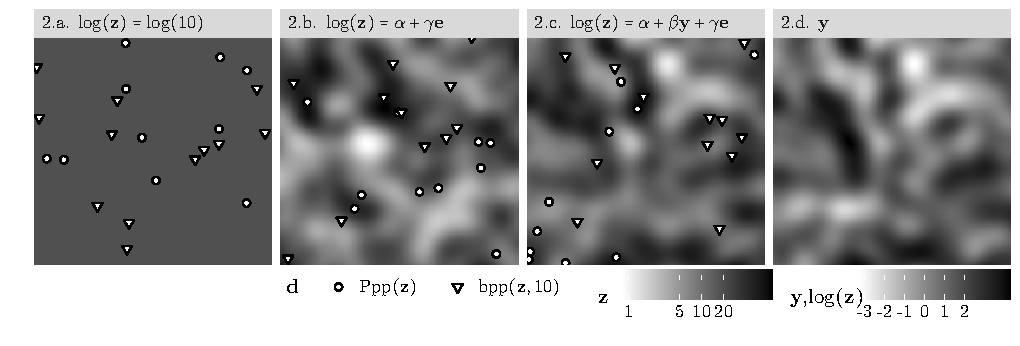
\includegraphics{fig/figure2.pdf}
    \vspace{-1cm}
    
    
    \footnotesize{
    
%
Sub-figures correspond to the  heatmap of a design variable $\desvar$ (Sub-figures 2.a, 2.b, 2.c) to the heatmap of $\signal$ (Sub-figure 2.d) and the plot of the samples (circle and triangle dots) drawn according to the two different designs. The values of $(\alpha, \beta ,\gamma)$ for each sub-figure are: 2.a: $(\log(10),0,0)$, 2.b:$(\log(10)-(0.5^2+0.3^2),0,\sqrt{0.5^2+0.3^2})$, 2.c: $(\log(10)-(0.5^2+0.3^2),0.5,0.3)$.}
%\end{mdframed}

\end{figure}

\begin{figure}[H]
%\begin{mdframed}
\caption{Joint and marginal densities of $\desvar$ and $\signal$}\label{fig:jointmarginaldensitiesYZ}
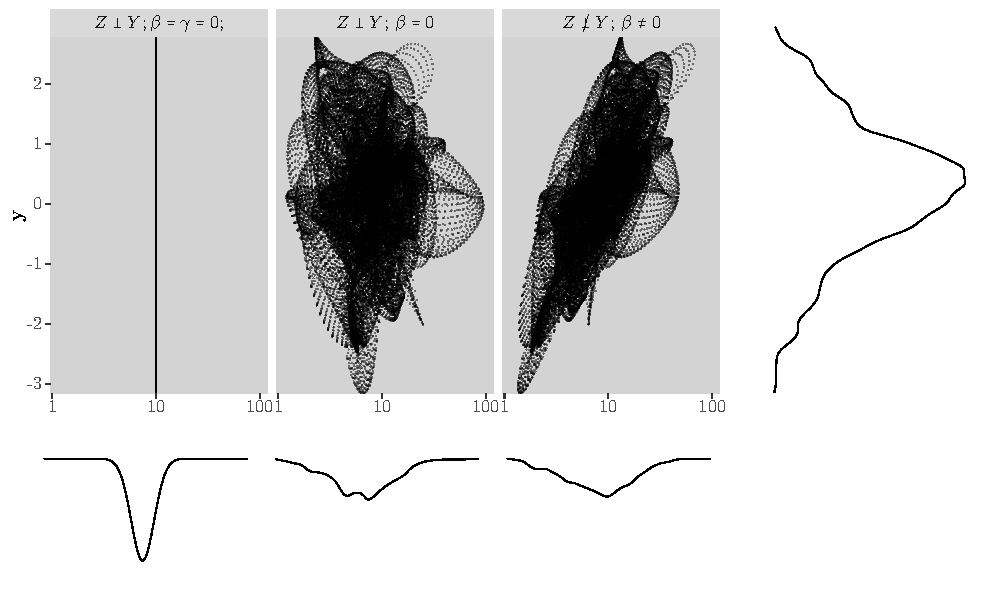
\includegraphics{fig/figure3.pdf}
\footnotesize{
 Each sub-figure contains the scatter plot of  $\left\{\left(\desvar[\position],\signal[\position]\right):\position\in\mathrm{Grid}\right\}$, where $\mathrm{Grid}$ is a regularly spaced grid of $\Pop$. The values of $(\alpha, \beta ,\gamma)$ for each Sub-figure are: 3.1: $(\log(10),0,0)$, 3.2:$(\log(10)-(0.5^2+0.3^2),0,\sqrt{0.5^2+0.3^2})$, 3.3: $(\log(10)-(0.5^2+0.3^2),0.5,0.3)$. The vertical axis corresponds to $\signal$, the vertical to $\desvar$. The marginal plots correspond to the density of $\desvar$ (right margin) and to the densities of $\signal$ (bottom margins).}
%\end{mdframed}
\end{figure}




\subsection{Observations}
The observation consists of the realisations of the random variables $\Sample$ and $\Signal[\Sample]$. 
%$(\Sample[\ell],\Signal[\Sample[\ell]])_{\ell\in\{1,\ldots,\Sampleindex}$
%Observations $(\Sample,\Signal[\Sample])=(\Sample[\ell],\Signal[\Sample[\ell]])_{\ell=1,\ldots,n}$ can be seen as a point process in $\Pop\times\SignalSpace$ and its intensity is defined as the Radon Nikodym derivative of $\Intensity_S$ with respect to the measure $\dominantU\otimes\dominantY$.

